\documentclass[8pt,xcolor=dvipsnames,compress]{beamer}
\usepackage{multimedia}
\usepackage{pcelab_theme}
\usepackage{mathtools}
\usepackage{multirow}
\usepackage{graphicx}
\usepackage{pcelab_style}
\usepackage{hyperref}
%\usepackage[algoruled,longend]{algorithm2e}
\usepackage{array}
\usepackage{graphicx}
\graphicspath{ {./images/} }
\usepackage{amsmath}
\newcolumntype{C}{>{\centering\arraybackslash} m{1000.3in} }
\newcolumntype{M}{>{\centering\arraybackslash} m{1000.in} }
\everymath{\displaystyle}
\long\def\/*#1*/{}

%\beamertemplatenavigationsymbolsempty
%\usepackage[square,numbers]{natbib}
\usepackage{tcolorbox}
\usepackage{rotating}
\usepackage{xcolor}
\usepackage[export]{adjustbox}
\usepackage{caption}
\usepackage{subcaption}
\newcommand{\bs}{\boldsymbol}
\newcommand{\thetab}{\boldsymbol\theta}

%===============================================================================
% 					 Presentation Title and Author  
%===============================================================================
\title[Fall,2019]{
TCN Implementation Example Pytorch}
\subtitle{Semester: Summer, 2024}

\author{Md Azharul Islam}

\institute[UB]{Advisor:  Dr. Danial Faghihi\\University at Buffalo\\}
    \titlegraphic{
\includegraphics[width=3cm]{PCE_logo1.png}}

\date[\today]{\today}


\begin{document}
% \titlegraphic{\hfill\includegraphics[height=1.5cm]{logo.pdf}}
\maketitle

\begin{frame}[fragile]{Dataset}
\footnotesize
\textbf{Hourly energy demand generation and weather:}\\
From the paper "Tackling Climate Change with Machine Learning", forecasting in energy markets is identified as one of the highest leverage contribution areas of Machine/Deep Learning toward transitioning to a renewable based electrical infrastructure.

This dataset contains 4 years of electrical consumption, generation, pricing, and weather data for Spain. Consumption and generation data was retrieved from ENTSOE a public portal for Transmission Service Operator (TSO) data. Settlement prices were obtained from the Spanish TSO Red Electric España. Weather data was purchased as part of a personal project from the Open Weather API for the 5 largest cities in Spain and made public here.

\begin{figure}[htpb]
        \centering
        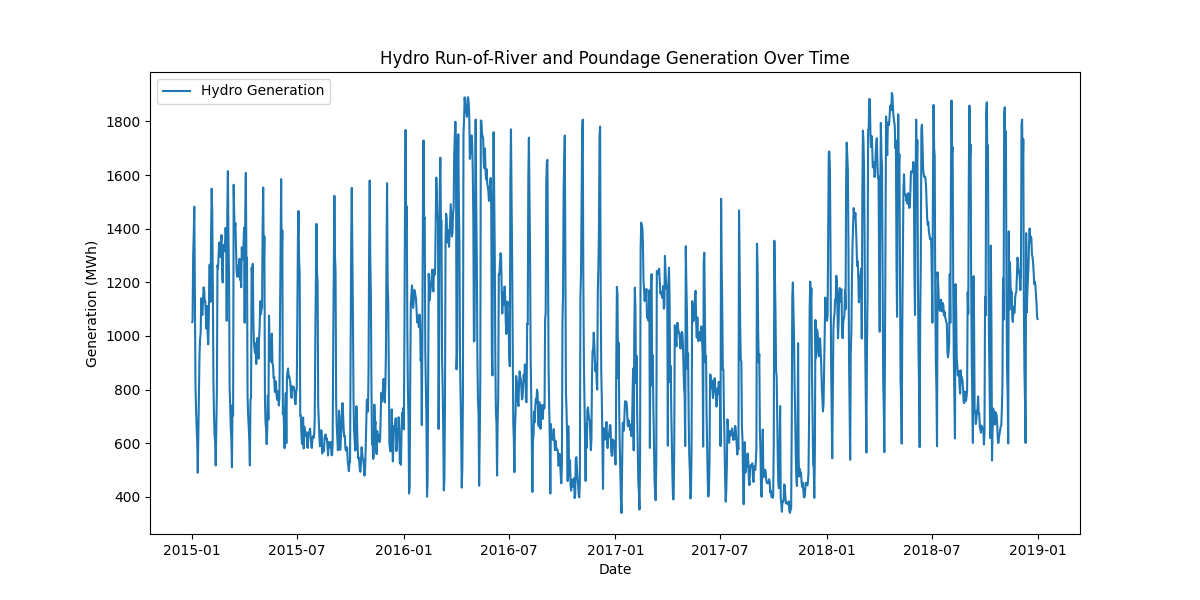
\includegraphics[scale=0.30]{figures1/full_data.png}
        \caption{One week prediction with some more training data}
\end{figure}
\end{frame}

\begin{frame}{Comparison of TCN Architectures}
\footnotesize
\begin{table}[h!]
\centering
\caption{Encoder Decoder TCN Architecture Summary}
\begin{tabular}{|c|c|c|}
\hline
\textbf{Component} & \textbf{Number of Layers} & \textbf{Components per Layer} \\
\hline
Chomp1d & 1 per TemporalBlock & N/A \\
\hline
TemporalConvNet & 3 & TemporalBlock \\
\hline
TemporalBlock & 2 & \begin{tabular}[c]{@{}c@{}}Conv1d (Weight Norm)\\ Chomp1d\\ ReLU\\ Dropout\end{tabular} \\
\hline
TCNEncoder & 1 & \begin{tabular}[c]{@{}c@{}}TemporalConvNet (with 1 input channel)\\ Permute Layer\end{tabular} \\
\hline
TCNDecoder & 3 & \begin{tabular}[c]{@{}c@{}}Conv1d\\ ReLU\\ Dropout\\ \hline Final conv1d\end{tabular} \\
\hline
\end{tabular}
\end{table}

\begin{table}[h!]
\centering
\caption{Plain TCN Architecture Summary}
\begin{tabular}{|c|c|c|}
\hline
\textbf{Component} & \textbf{Number of Layers} & \textbf{Components per Layer} \\
\hline
Chomp1d & 1 per TemporalBlock & N/A \\
\hline
TemporalBlock & 2 & \begin{tabular}[c]{@{}c@{}}Conv1d (Weight Norm)\\ Chomp1d\\ ReLU\\ Dropout\\ \hline Downsample (Optional)\\ ReLU\end{tabular} \\
\hline
TemporalConvNet & 3 & TemporalBlock \\
\hline
TCN & 1 & \begin{tabular}[c]{@{}c@{}}TemporalConvNet\\ Linear Layer\end{tabular} \\
\hline
\end{tabular}
\end{table}

\end{frame}

\begin{frame}[fragile]{Hyper-parameters}
\footnotesize
\textbf{The hyperparameters used for training}\\
Batch size = 16 \\
Dropout ratio= 0.2 \\
Epochs = 10 \\
Kernel (filter) size = 3 \\
Sequence length = 7 \\
Learning rate = 0.001 \\
Optimizer = Adam \\

\end{frame}

\begin{frame}[fragile]{Training and Testing}
\footnotesize
\textbf{Encoder-Decoder TCN Training and Testing Results}\\
Epoch 1, Loss: 0.6989267638160123\\
Epoch 2, Loss: 0.1672599609527323\\
Epoch 3, Loss: 0.11022111835579078\\
Epoch 4, Loss: 0.0860006758529279\\
Epoch 5, Loss: 0.07287092336143057\\
Epoch 6, Loss: 0.06404010077110595\\
Epoch 7, Loss: 0.05766288755047652\\
Epoch 8, Loss: 0.05555434017959568\\
Epoch 9, Loss: 0.052257696270114846\\
Epoch 10, Loss: 0.049869451568358474\\
Test set: Average loss: 0.025551\\
\\
\textbf{Plain TCN Training and Testing Results}\\
End of Epoch  1         Learning rate: 0.0010   Loss: 0.814014\\
End of Epoch  2         Learning rate: 0.0010   Loss: 0.483615\\
End of Epoch  3         Learning rate: 0.0010   Loss: 0.290282\\
End of Epoch  4         Learning rate: 0.0010   Loss: 0.250012\\
End of Epoch  5         Learning rate: 0.0010   Loss: 0.234309\\
End of Epoch  6         Learning rate: 0.0010   Loss: 0.221363\\
End of Epoch  7         Learning rate: 0.0010   Loss: 0.215366\\
End of Epoch  8         Learning rate: 0.0010   Loss: 0.209273\\
End of Epoch  9         Learning rate: 0.0010   Loss: 0.204705\\
End of Epoch 10         Learning rate: 0.0010   Loss: 0.198154\\
Test set: Average loss: 0.404127
\end{frame}


\begin{frame}[fragile]{Model 1: Encoder decoder TCN Results}
\footnotesize

\begin{figure}[htpb]
    \centering
    \begin{subfigure}[b]{0.65\textwidth}
        \centering
        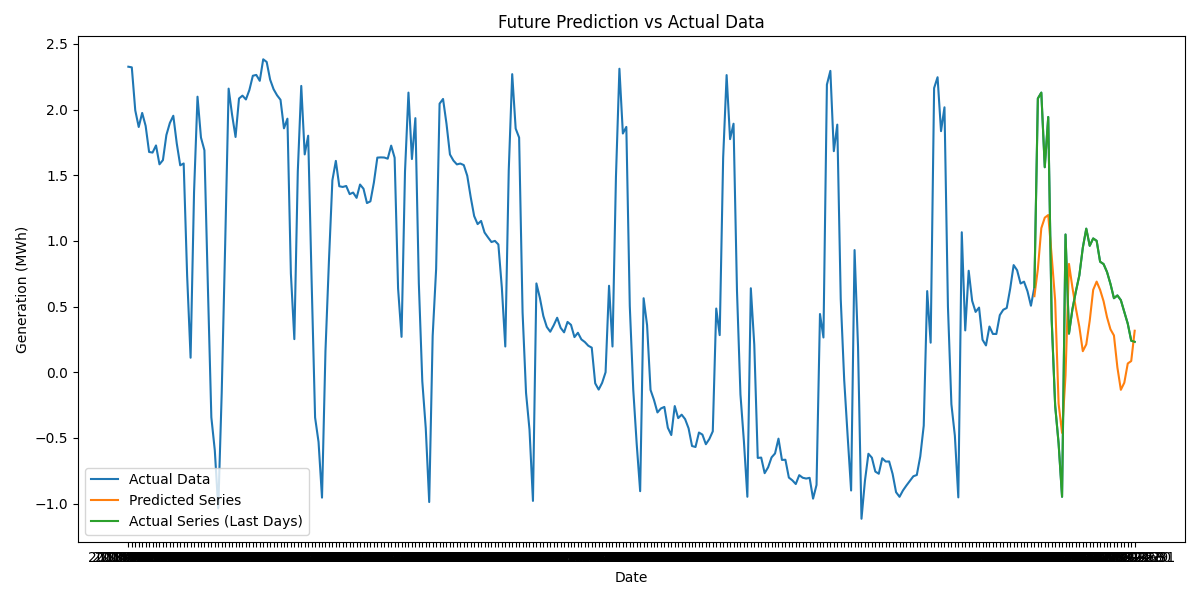
\includegraphics[scale=0.20]{figures1/ED_pred_more.png}
        \caption{30 Days prediction with some training data}        
    \end{subfigure}
    \begin{subfigure}[b]{0.65\textwidth}
        \centering
        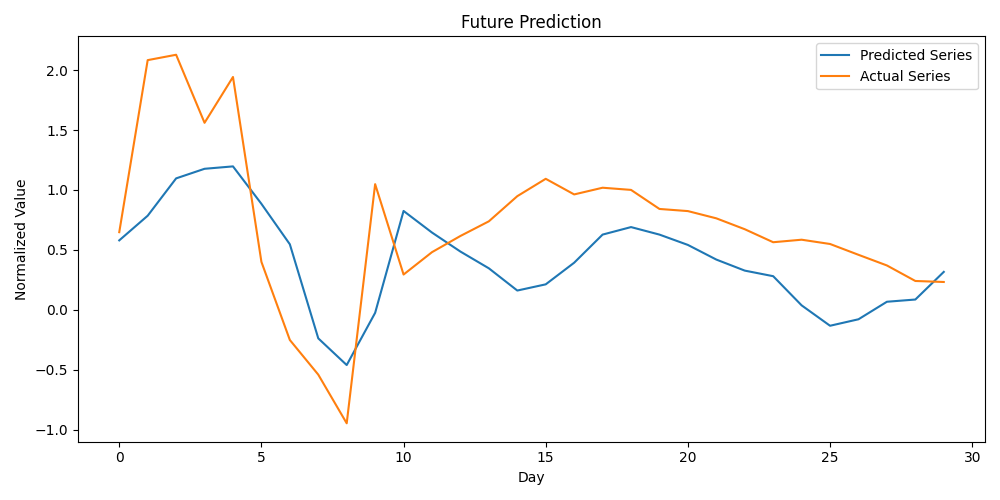
\includegraphics[scale=0.25]{figures1/ED_30days_pred.png}
        \caption{30 Days Prediction 10 epochs}
    \end{subfigure}
    \label{fig:eigenvalue_decay}
\end{figure}

\end{frame}

\begin{frame}[fragile]{Model 2: Single TCN Results}
\footnotesize

\begin{figure}[htpb]
    \centering
    \begin{subfigure}[b]{0.65\textwidth}
        \centering
        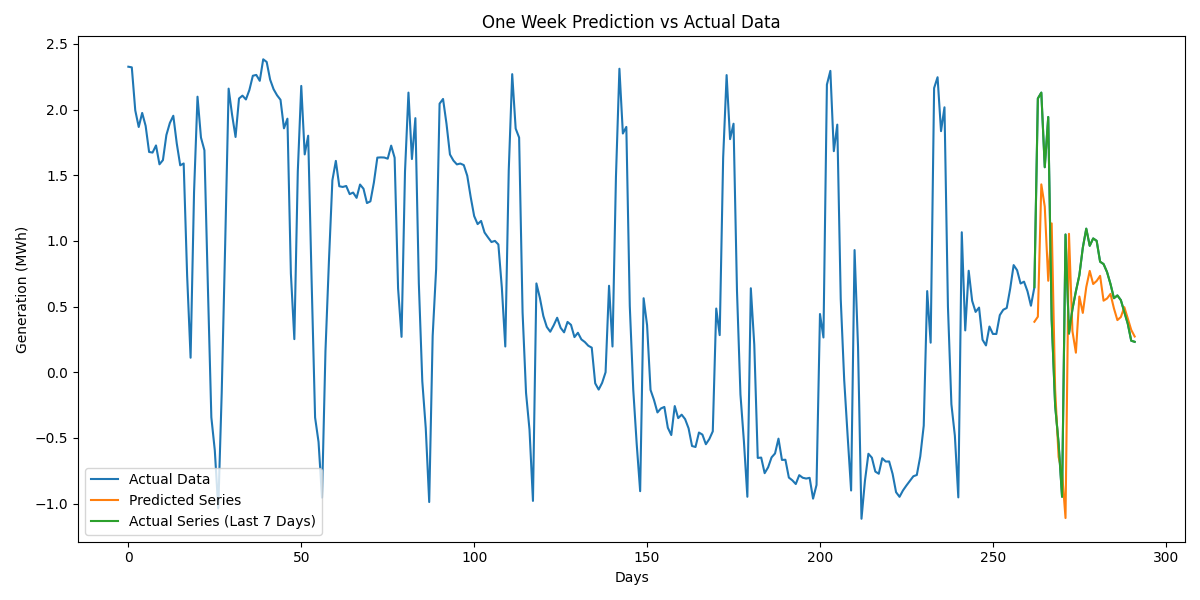
\includegraphics[scale=0.20]{figures1/TCN_pred_more.png}
        \caption{30 Days prediction with more training data}        
    \end{subfigure}
    \begin{subfigure}[b]{0.65\textwidth}
        \centering
        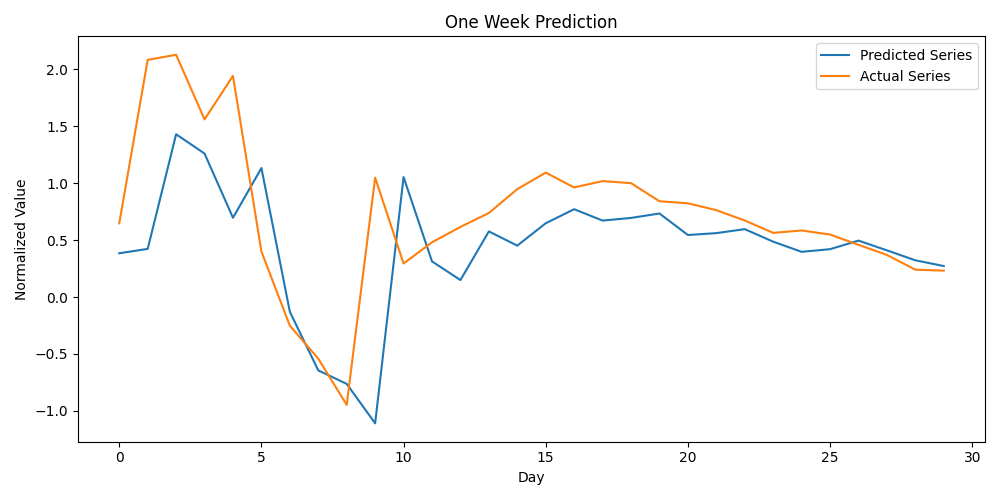
\includegraphics[scale=0.25]{figures1/TCN_pred_30.png}
        \caption{30 days prediction 10 epochs}
    \end{subfigure}
    \label{fig:eigenvalue_decay}
\end{figure}

\end{frame}


\begin{frame}[fragile]{Results 100 epochs}
\footnotesize

\begin{figure}[htpb]
    \centering
    \begin{subfigure}[b]{0.65\textwidth}
        \centering
        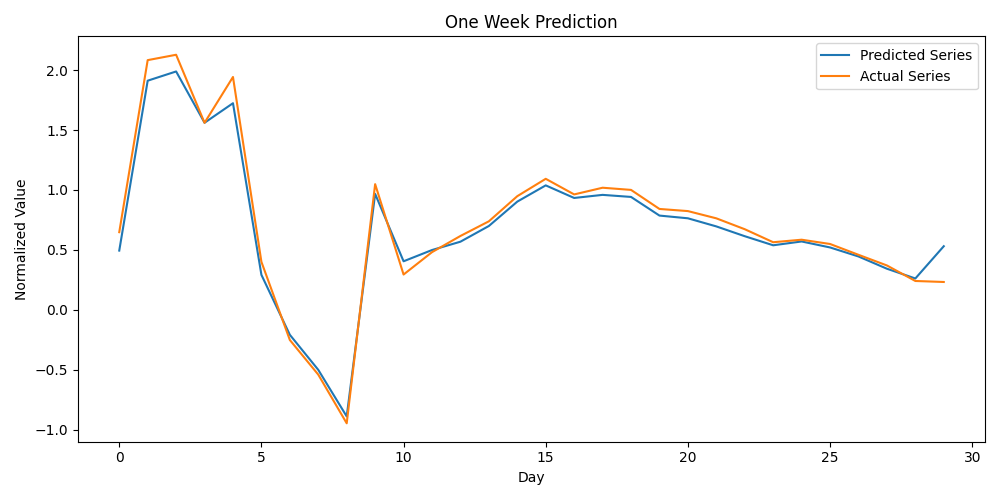
\includegraphics[scale=0.25]{figures1/ED_30days_100epochs.png}
        \caption{30 Days prediction with Encoder Decoder}        
    \end{subfigure}
    \begin{subfigure}[b]{0.65\textwidth}
        \centering
        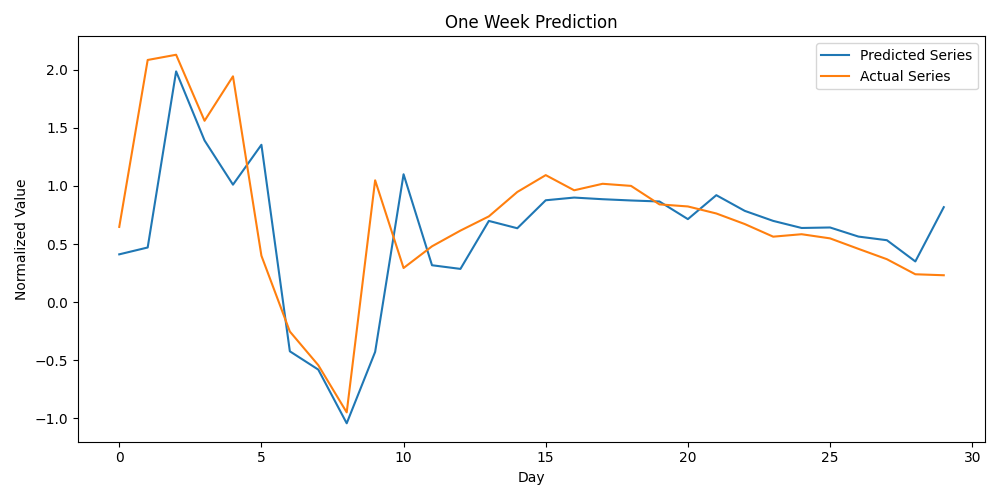
\includegraphics[scale=0.25]{figures1/30days_100epoch_TCN.png}
        \caption{30 days prediction with plain TCN}
    \end{subfigure}
    \label{fig:eigenvalue_decay}
\end{figure}

\end{frame}

\begin{frame}[fragile]{Layer output dissection}
\footnotesize

\begin{figure}[htpb]
    \centering
    \begin{subfigure}[b]{0.65\textwidth}
        \centering
        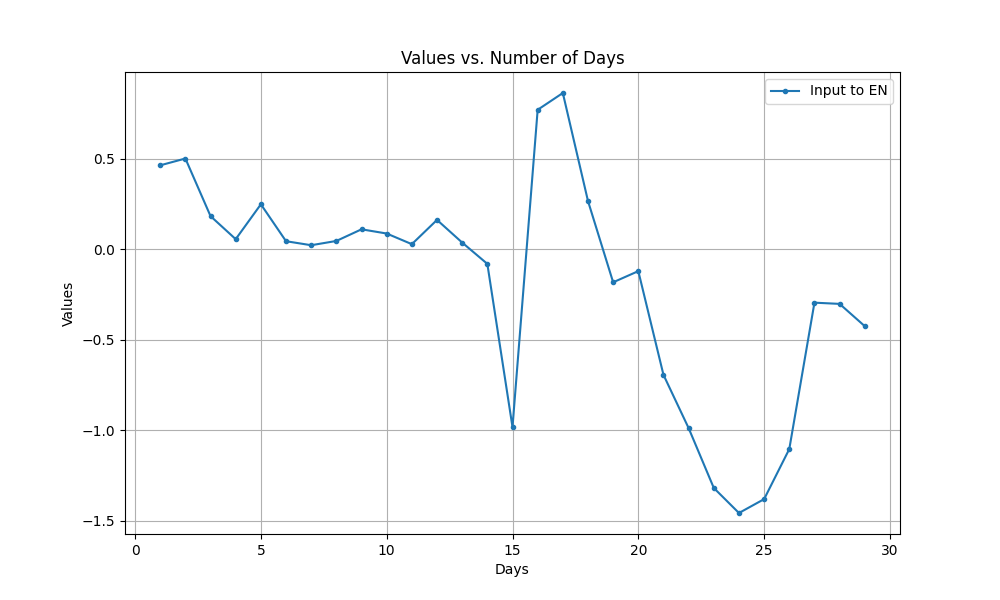
\includegraphics[scale=0.25]{figures1/input_to_encoder.png}
        \caption{30 Days prediction with Encoder Decoder}        
    \end{subfigure}
    \begin{subfigure}[b]{0.65\textwidth}
        \centering
        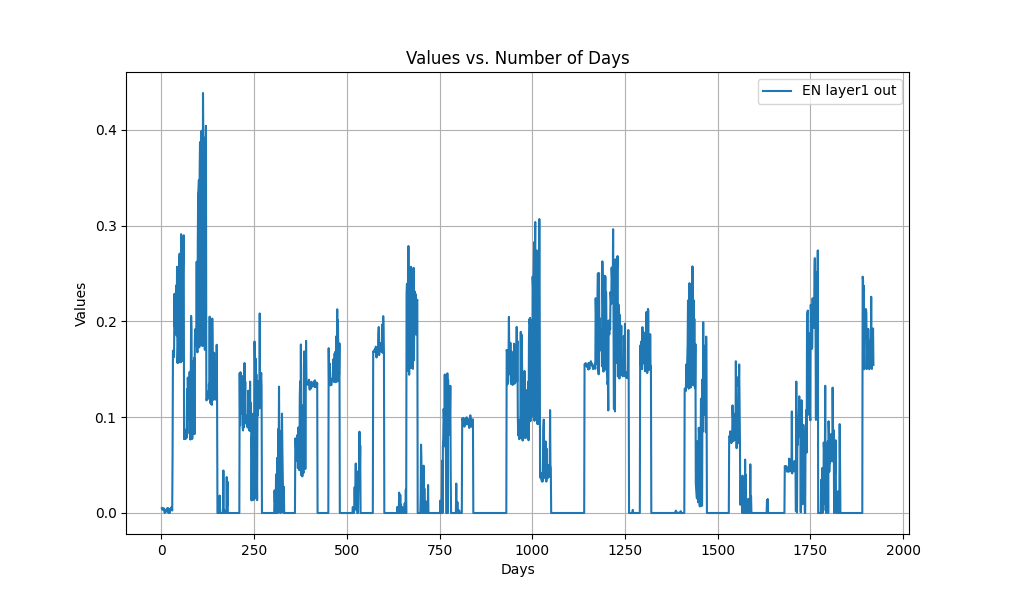
\includegraphics[scale=0.25]{figures1/Encoder_layer1_output.png}
        \caption{30 days prediction with plain TCN}
    \end{subfigure}
    \label{fig:eigenvalue_decay}
\end{figure}

\end{frame}


\begin{frame}[fragile]{Layer output dissection}
\footnotesize

\begin{figure}[htpb]
    \centering
    \begin{subfigure}[b]{0.65\textwidth}
        \centering
        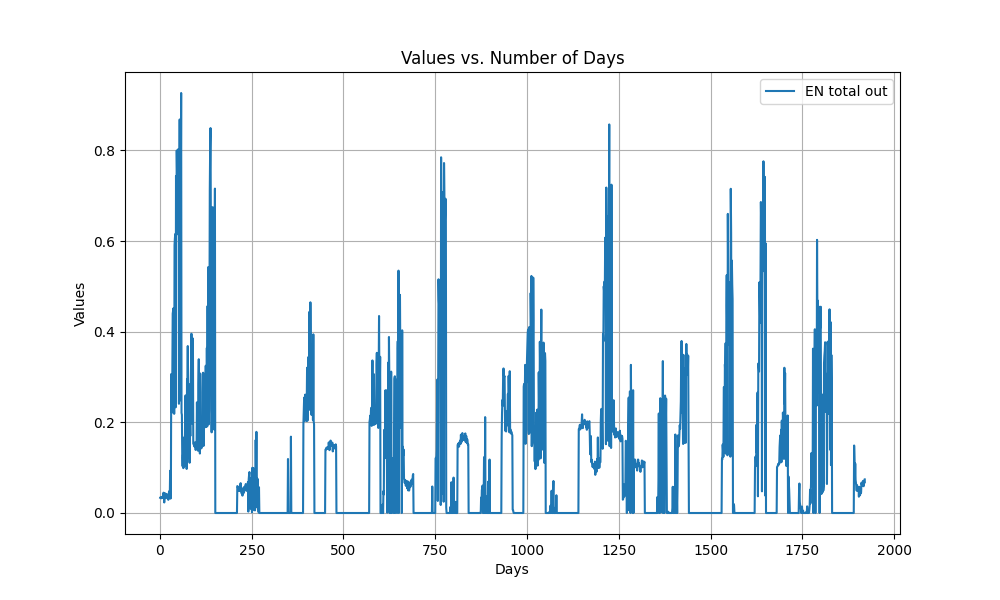
\includegraphics[scale=0.25]{figures1/Encoder_output.png}
        \caption{30 Days prediction with Encoder Decoder}        
    \end{subfigure}
    \begin{subfigure}[b]{0.65\textwidth}
        \centering
        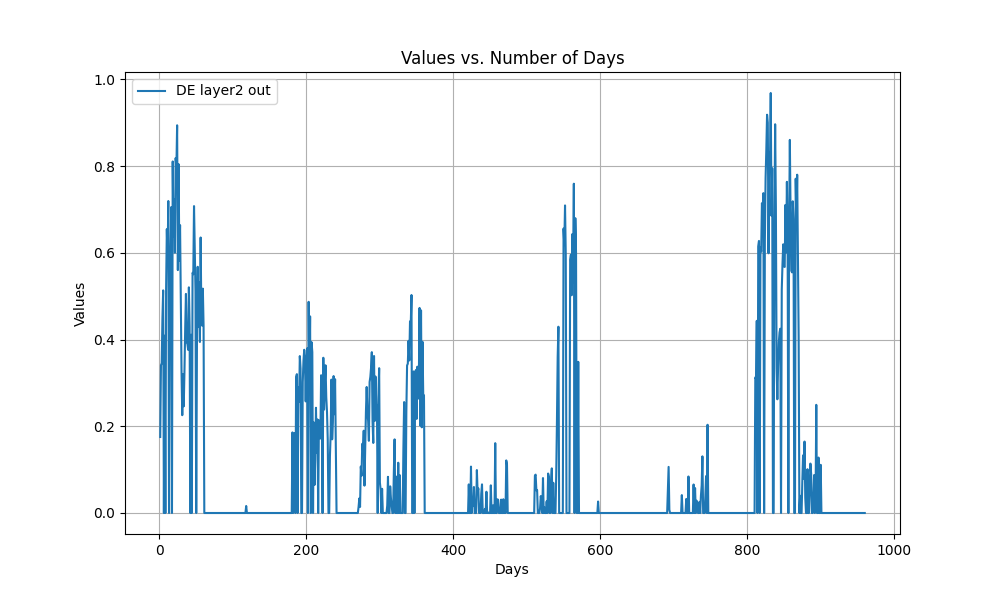
\includegraphics[scale=0.25]{figures1/decodr_layer2_output.png}
        \caption{30 days prediction with plain TCN}
    \end{subfigure}
    \label{fig:eigenvalue_decay}
\end{figure}

\end{frame}

\begin{frame}[fragile]{Layer output dissection}
\footnotesize

\begin{figure}[htpb]
    \centering
    \begin{subfigure}[b]{0.65\textwidth}
        \centering
        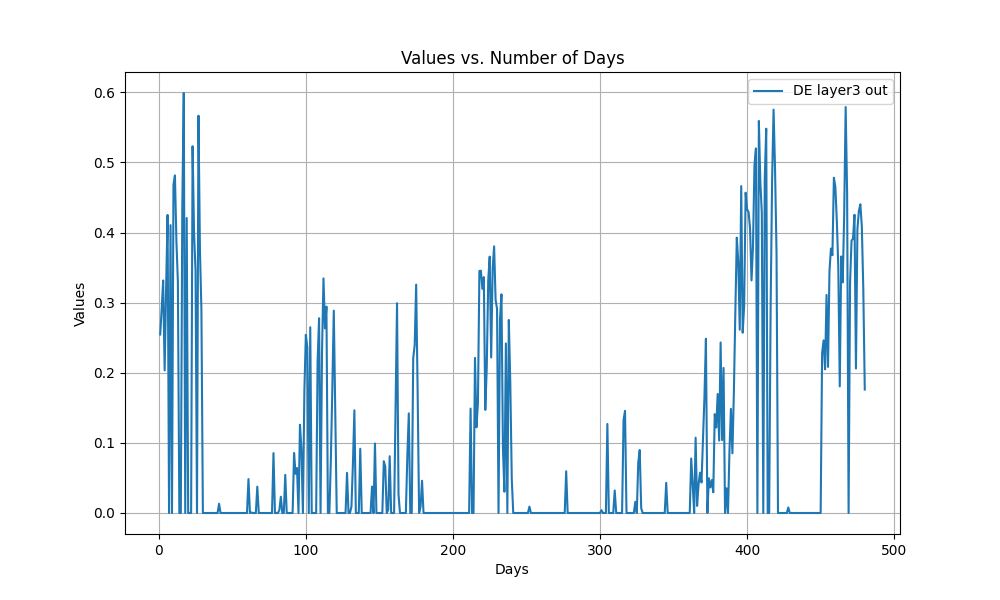
\includegraphics[scale=0.25]{figures1/decoder_layer3_output.png}
        \caption{30 Days prediction with Encoder Decoder}        
    \end{subfigure}
    \begin{subfigure}[b]{0.65\textwidth}
        \centering
        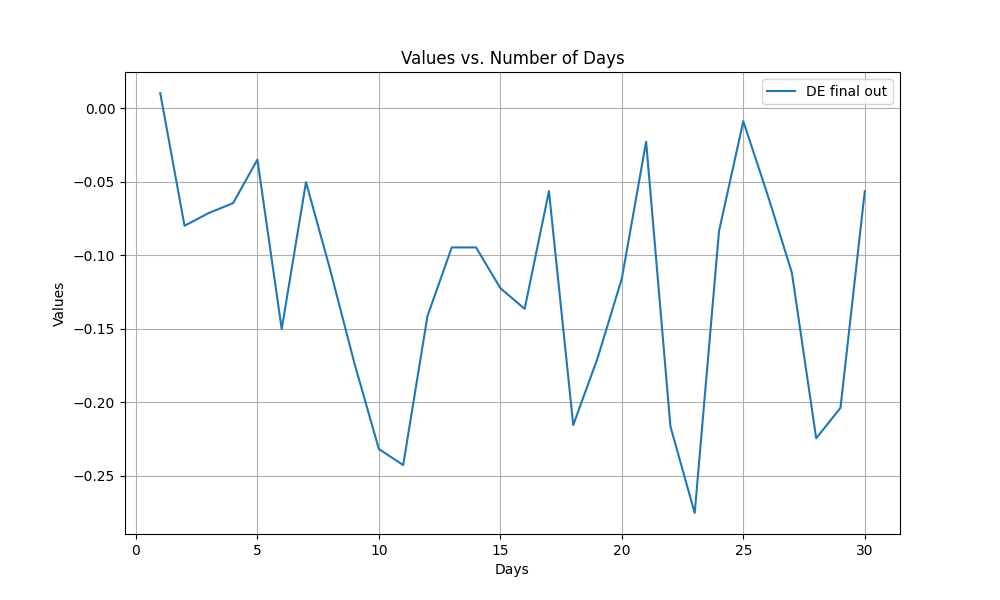
\includegraphics[scale=0.25]{figures1/Deocder_output.png}
        \caption{30 days prediction with plain TCN}
    \end{subfigure}
    \label{fig:eigenvalue_decay}
\end{figure}

\end{frame}


\end{document}